\chapter{Implementation}
\label{cha:implementation}

In the following sections we will describe implementation details, where implementation was different from the concept and motivate our decision. 
We will further mention challenges and problems and how we overcome thous. 

\section{Core-Logic}
Blockchain-Identity is always focus around two actors: The user and his interaction with the blockchain and identity providers and their interaction with the user in an on- and off-blockchain fashion. We model our system in the same way but needed to make some specifications for the provider service which comes with two different motivations and rights:

\begin{itemize}
\item \textbf{Normal Provider}: Holds domain specific personal data about their customers that are not exposed to the outside world. They have an interest in requesting user data to extend their system and to make new costumer registration easier. This services are untrusted and can not write to the blockchain. However they can read from the blockchain to verify transactions or extract information out of it. In general everyone can setup a provider service and request user data. They don’t need to be verified in any kind. 
\item \textbf{Government}: Single trusted entity that holds verifiable citizen information. This information are backed by the representative citizen office or other federal trusted institutions. The government usually verifies user data.
The government service is the only service that can read and write to the blockchain. 
The client application, on the other hand, has read and write access to the blockchain and can interact with this providers.
This following sections describes the different provider/client applications and their interactions with the other components: frontend, Etherem-Blockchain-Adapter (EBA) and the database.
\end{itemize}

\subsection{Motivation}
Since we are dealing with services which are providing user data we decided to implement a normal client-server architecture. Here we can use all the advantages TCP is providing us like transport layer encryption with SSL/TLS and the reliability/inorder-delivery TCP comes with. Where we would have to deal with our own encryption-scheme if we would use UDP with peer-to-peer communication and port discovery, even if peer-to-peer communication seems like the more fitting solution since we are already in the domain of blockchain and decentralized applications. 

Choosing a client-server architecture comes with the drawback that the government service can not notify the client about incoming messages. The communication via the blockchain is not possible since the provider have not permission to write to it (it would also not be feasible regarding the cost writing to the blockchain comes with). To overcome this challenge we implemented a discovery service where each components registers to on bootstrap. (See section \ref{sec:discoveryService}).

We further decided to design our services RESTful (Representational state transfer). This in mind spring boot\footnote{\url{https://projects.spring.io/spring-boot/}} is a good choice in the Java domain for rapid prototyping. Spring boot also offers good integration for database adapters and spring security\footnote{\url{https://projects.spring.io/spring-security/}} a authentication and authorization framework. 

\subsubsection{Tools and Technologies}
Besides Spring Boot and Spring Security we further committed us to the following technology stack:

\begin{itemize}
\item Springfox\footnote{\url{https://springfox.github.io/springfox/}}: A API documentation framework. Additionally it is specifically designed for Spring Boot.
\item Feign\footnote{\url{https://github.com/OpenFeign/feign}}: Framework that make writing API calls easier. You only need to provide an interface and specify it with annotations to produce a HTTP request to a specific domain. Mapping and error handling is mostly done by Feign. 
\item Lombok\footnote{\url{https://projectlombok.org/}}: Lombok reduces the boilerplate code in Java by directly translating data or logging annotation into java byte code. It helps us to reduce the size of our models to a minimum by obscuring the setter, getter and constructors. 
\item Bouncy Castle\footnote{\url{https://www.bouncycastle.org/java.html}}: The unofficial default cryptographic library for Java. It implements the Java security provider interface and provides a functions like RSA encryption or signature mechanism.
\item Zxing\footnote{\url{https://github.com/zxing/zxing}}: Library to generate QR- and bar-codes. 
\item Web3j\footnote{\url{https://web3j.io/}}: Library providing the Ethereum adapter. (More in section \ref{sec:eba}. In this section this library is mainly used to generate ECDSA (Elliptic Curve with Digital Signature Algorithm) signatures. 
\end{itemize}

Further the following testing technologies are used:

\begin{itemize}
\item AssertJ\footnote{\url{https://joel-costigliola.github.io/assertj/}}: A fluent assertion semantic for Java. 
\item Mockito\footnote{\url{http://site.mockito.org/}}: Mocking library to make unit and rest test more modular and encapsulated from outstanding components. 
\item Spring Boot Test\footnote{\url{https://docs.spring.io/spring-boot/docs/current/reference/html/boot-features-testing.html}}: Integration test framework for Spring Boot. 
\end{itemize}

\subsection{Claims}
The Blockchain-Identity is centralized around user claims. Claims are atomic statements of personal information, that can be made about a person. They describe units of information you receive if you continue to cut bigger personal information chunks into smaller onces. We introduce 5 different claim types: 

\begin{itemize}
\item \textbf{Boolean}: Boolean-claims are claims that can be answered with a simple yes or no answer.
Example: "Has HVI?" 
\item \textbf{String}: String-claims are the most common onces. They shell not be longer then one word or name. 
Example: "Which street lives Bob in?"
\item \textbf{Number}: Number-claims hold numbers (in double representation) as values. 
Example: "What is Bobs ZIP code?"
\item \textbf{Date}: Date-claims relate to claims that refer to a specific time or date. They are saved as LocalDateTime objects.
Example: "When was Bob born?"  
\item \textbf{Object}: All other claims that are not representable with the above definitions need to be saved as generic objects. This may be lists of claims, or even more complex representations like whole documents. Since we decided that in our prototype you can break down every claim in a subset of the above definition, this claim is lacking support in a closure related context. 
Example: "What is Bobs whole medical record?"
\end{itemize}

Claims are structured in the same way in every implemented system. A claim in its core consists of an identifier (ID), type and value. The ID defines a unique string that is well known and is strictly bound to a claim type. 
An overview about all current defined claim IDs can be found in appendix \ref{appendix:claimID}. Claim IDs are on propose defined as strings and not an enums since they shell be expendable and each provider shell be able to include their own claim IDs if non of the defined claim IDs fits their needs. With each new defined claim ID a claim type needs to be chosen. On runtime this type is validated against the claim value and if the value is not from the same type an exception will raise. 

The claim type is bound to claim operations. Claim operations are logical operations that can be interpreted by the closure expression engine. We will explain in detail how that work in section \ref{sec:closure}. 

The claim value is implemented as an universal type (class object) to be as generic as possible. Some could imagine that it shell be a generic (introduced since Java 1.6), but they are hard to serialize and deserialize. Since generics are defined on compile time and claims are often read from and to the database as well as send via the network, the overhead of type determination would be larger then just parsing it into an object and checking the type manual. 

Claims also hold some meta information about who is the issuer (reference to the provider, original issuing this claim) of this claim, and a modification date which gets updated each time a claim is changed. The modification date enables us to see if a claim is outdated and needs to be updated again. Claims are of nature signed. The signature is generated by the provider validated the claim. 

\subsection{Components}
\begin{figure}
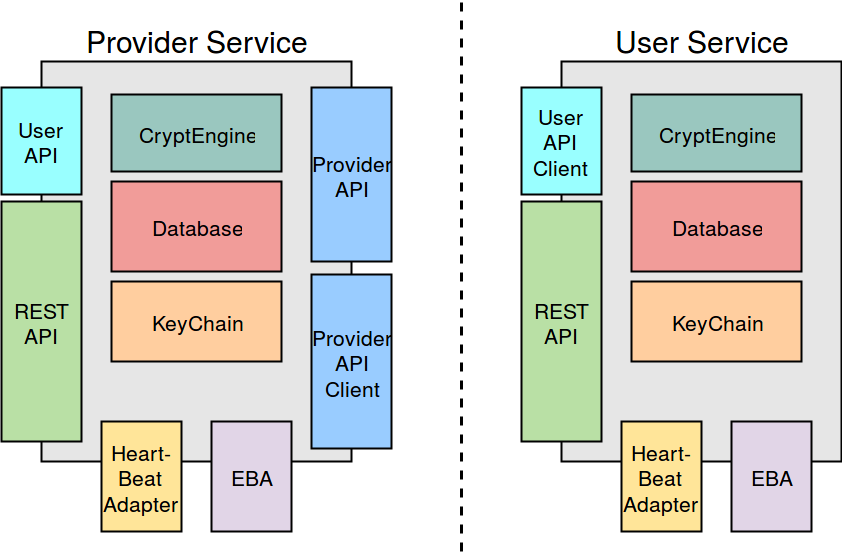
\includegraphics[width=0.7\textwidth]{impl/ComponentDiagram.png}
\centering
\caption{Overview about the components of an individual service and their exposed endpoints. On the left side is the provider service displayed, serving, additional to the user service, a provider API and provider API client. On the right side is the user service located implementing the client API client.}
\label{fig:componentDiagram}
\end{figure}

In figure \ref{fig:componentDiagram} you can see an overview about the core components of the provider and user service. All boxes that are drown over the border are representations of exposed endpoints or clients and inside the box are the internal components listed.

\subsubsection{Internal components}
The crypt engine is the main framework for encrypting, decrypting, signing, validating signatures and generating secure hashes. It provides methods for symmetric and asymmetric encryption. It uses bouncy castles as security provider to generate keys and handle cryptography. To generate elliptic curve signatures it uses the framework provided by web3j. 

We are using spring data to provide a very easy interface to couchbase, our database storage (section \ref{sec:database}). The keychain is the a session object holding the RSA key-pair, EC key-pair and some other meta information about the current state of the service. This objects gets cleared if the services logs out and restored if the service logs in (section \ref{sec:registerContract}). 

\subsubsection{User API}
\label{sec:userAPI}
The user API provided by a provider service and requested by the user service defines the central entry point of client requests to a provider. The user and the provider API (section \ref{sec:providerAPI} is implemented as a normal Java interface. The provider service is implementing this interface and mapping the defined methods to REST endpoints which then are bounded to a predefined paths. The user service on the other hand, extends this interface in a new interface which then serves as a Feign adapter bound to the same predefined paths. This is really convenient because Feign needs an annotated interface to build an REST client out if it. We only have to bind Feign to the same resources paths the provider is exposing so that they can communicate to each other. 

Using this interface for the client and server side implementation allows us to easy extend the API without leaving many room for errors. Changing one endpoint on server side will directly effect the implementation on client side. 

\subsubsection{Provider API}
\label{sec:providerAPI}
The provider API is a unified interface which each provider is offering in form of REST endpoints. Each provider builds also a Feign client (see section \ref{sec:userAPI}) to talk to other providers.  Via this API provider an interact with each other provider to exchange information or offering services. Notably is that each request needs to be authenticated via a SignedRequest (see section \ref{sec:ecdsa}) to ensure that only authenticated entities request this API. 

\subsubsection{REST API}
The general REST API is the connection to the frontend. Here the frontend can ask for user resources and claims to display them a web administrator or the end user. This requests are authenticated via “basic authentication”, a mechanism which is not optimal because the password and user name is transmitted in plain text if no transport layer encryption is used. The plan was to change this mechanism to a more secure scheme like Json-Web-Token (JWT, signature based) authentication, but that would require changes in other components and was also out of scope of the focus of this project. 

\subsubsection{HeartBeatAdapter and EBA}
The Ethereum Blockchain Adapter (EBA) is the entry point to communicate with the blockchain. We defined an interface (EBAInterface) between the blockchain component and the core-logic to make the core-logic ethereum independent. Relate to the section \ref{sec:eba} where everything related to the blockchain is explained. If we for some reason decide to use a different blockchain implementation we could reimplement the EBAInterface.

The HeartBeatAdapter is the connection to the Discovery Service (section \ref{sec:discoveryService}). A service can register itself to the discovery service, create or subscribe to new beats.

\subsection{Notable methods}
The follow sections describe challenges that occurred during development and how they were solved. 

\subsubsection{Serializing and deserialization of arbitrary objects}
\label{sec:serialobject}

Serialization of arbitrary objects is a challenge in systems where the order of serialization is imported (in our case: building a signature via hashing over the serialization outcome). A common serialization method is the JSON-String serialization, where an arbitrary object state gets converted into a JSON representation. This can be done by (for example) the Jackson object mapper\footnote{\url{https://github.com/FasterXML/jackson}}. Different configuration of the object mapper makes it difficult to receive the same serialization outcome on each system. To overcome this problem, we defined a universal object mapper configuration for Spring, crypt- engine and database. For example we need define the order  in which each field of the object gets serialized. The big advantage by using the JSON-string serialization is that we don’t have to binary encode the signed object on transmitting it to the frontend to ensure its integrity. We only have to make our serialization configuration public so that every party, obtaining a signed JSON, can verify its authenticity.

An alternative approach was to use Javas serialization API. Classes that implement "Serializable" will then be converted to a stream which then can be collected to a byte array. Since Java serialization will take care of the serialization order of fields by itself we don’t have to bother with that. 

However, we need to find a unique way to serialize objects since building a hash-based signature via objects must be done always in the same way, no matter on which system the signing or verification of the signature is happening. We decided to use JSON serialization approach (with explicitly defining the order in which properties shell be serialized) since it is language independent, easier to implement and to debug, even if it is not as efficient as raw byte representation. How exactly signatures are build and verified is described in the next section \ref{sec:ecdsa}. 

The implementation of sets in the Java Virtual Machine needed also consideration. Sets are of nature unordered and it depends on the order of object initialization on the heap to define the real order the elements are returned in. If you want the same order of object each time, you need to use lists. Building a hash over an object holding sets is obviously a bad idea since the order of attributes may be different from system to system, so the hash will be a different too.  

Another problem related to serialization was that variables of type "Object" will be converted into a string representation and on deseralization this string will not be converted back into the original type since "String" itself extends "Object". This became a problem on serialization of LocalDateTime values, which were not parsed back into a LocalDateTime (the other values that were serialized are primitive types and so were correctly parsed). 

To temporary handle the different conversions we implemented a "ValueHolder", a simple class separating LocalDateTime values from generic Object values. By converting explicit into a LocalDateTime the Jackson converter recognizes the string representation and deserialize it into the correct object representation. Future improvements can be made by including the target class of the serialized value as meta information, so that on deseralization the value can be parsed back to its original class. Additionally the object mapper needs to be adapted adequately. 

\subsubsection{ECDSA and Signed-Requests}
\label{sec:ecdsa}

Elliptic Curve Digital Signature Algorithm (ECDSA) in the SECP256k1 configuration is used by Bitcoin and Ethereum to sign transaction to the blockchain \cite{mayer2016ecdsa}. This ensures integrity and authenticity to the sender and the content of the transaction. But it does not provide confidentiality in any kind, since Bitcoin or Ethereum want to stay as transparent as possible. 
A ethereum address is the hexadecimal representation of the elliptic curve public key prepended with a “0x”. 

To populate this security properties also between services we use ECDSA also for inter service communication (and additionally TLS/SSL to enforce confidentiality\footnote{Due to time limitations that feature could not be implemented. See section \ref{sec:securityEvaluation} for more information}). This is done by generating a so called \lstinline{SignedRequest<T extends BasicEthereumDTO>}. This object can hold a generic payload that extends the BasicEthereumDTO and the EC Digital-Signature over this payload. The BasicEthereumDTO enforces that the ethereum address of the sender (similar to ethereum transactions) is included in the signature. This value can later be used to validate the signature. A signature is then build in the following way: 

\begin{enumerate}
\item The payload gets converted to a JSON as defined in section \ref{sec:serialobject}
\item A SHA-256 hash is build over the given serialized JSON
\item This hash will then be signed by the ECDSA using the private key (EC) of the signer
\item The resulting signature gets appended to the payload
\end{enumerate}

\noindent The receiver of this signed request can validate the signature by applying the following steps:

\begin{enumerate}
\item Serialize the payload into a JSON with the same object mapper configuration as used for serialization.
\item Create a SHA-256 hash over the generated JSON
\item Validate the provided signature against the computed hash. Interesting to know is that web3j validation does not yield a boolean flag indicating a valid signature, but a computed ethereum address which would fit the signature of the payload. 
\item We take this generated ethereum address to check it against the included ethereum address in the payload. If they are equal the integrity of the message is ensured. 
\item In the final step we have to validate that the ethereum address is indeed the sender of this request. This can be done off-blockchain for example by querying the database and see if the saved ethereum address matches the requesting one. If that also yields true the authenticity of the request is also ensured. 
\end{enumerate}

Please note that, to completely be secured against man-in-the-middle attacks we further need to encrypt the  signature asymmetric to make it tamper proof. Without that only users are secured against man-in-the-middle attacks since their ethereum address is verified and bound to their identity. However since provider are not verified they are attackable. TLS/SSL would also help us here. If the whole message would be encrypted an attacker first have to break TLS to change the signature. This only adds an layer of security but the problem remains that the providers EC key pair is not certificated. 
(An proposed solution to this problem is given in the next section.)

To validate and build signatures over Java objects we are using the Jackson object mapper module \lstinline{jackson-datatype-jsr310} in version \lstinline{2.8.10}. This module is further configuration to write time values as a time stamp in the ISO-8601 format. 

\subsection{Discovery Service}
\label{sec:discoveryService}
As mentioned in the previous section the Discovery Service is the result of a client-server architecture in a peer-to-peer environment. But it further serves additional purpose for holding and distributing RSA public keys, discovering domain names, where to find the exposed API and if the requested service is online. 

While all the stored information is public visible no sensitive data is exposed to the Discovery Service. It just provides connection information and serves as a message broker. Each stored entry needs to be signed by the author with the private key bound to his ethereum address. All unauthorized requests are rejected by the service. By ensuring the authenticity of each entry creation or update it is ensured that no service spoofing can happen. Only the holder of the private key bound to his ethereum address can update his connection information.

However, we need some kind of mechanism to verify the connection between ethereum address and provided URL to hinder URL spoofing. SSL-Ceritifcates or DNSSEC may help us here if we use the private key of the referenced public key (either in the certificate or stored in the DNSKEY entry) to sign the ethereum address. This would fill the missing trust in the provider ethereum address and make the system overall more secure against spoofing and man-in-the-middle attacks. It is left open for future work to implement this approach properly. 

\subsubsection{Beats}
\label{sec:beats}
Beats are the messages that are routed by the Discovery Service. A \textit{beat} is a small package containing an event type describing that kind of message it is and a subject field referencing the location where the new information is to find. Each beat is uniquely identified by the combination of recipient ethereum address and the current beat number (incrementing per beat). 

There are two types of subjects: The URL references a API endpoint where new or updates information are now present. The recipient is requested to request this API endpoint to update his information state. The other kind of subject is a ethereum address: The recipient is requested to query the blockchain for the given address to process the information stored at this address. 

On registration entities start to periodically (each 10 seconds) ping the Discovery Service to wait for new incoming beats. Since the discovery service itself is not a trusted entity, each beat gets verified before processing and it is checked that the signature matches the senders (provider/user) ethereum address.

The \lstinline{HeartBeatService} provides a very simple but powerful subscriber pattern to register to certain beats. Each sub system that wants to get notified on certain beats can implement a 
a lambda expression that gets called if a beat gets recognized. 

\subsubsection{PKI}
\label{sec:pki}

A Public-Key-Infrastructure (PKI) is an infrastructure to bound identities to public keys. This usually relay on trust in either a Certificate Authority or on other users trusting this public key. 

Since each entity stores also his RSA public key into the discovery service and sign this entry with his EC private key, the trust of the given RSA public key is tightly bound this EC key pair. If the RSA key gets stolen it can be simply replaced in the Discovery Service. If the EC key gets stolen both key pairs need to be regenerated. How we establish trust in the users EC key pair is explained in the next section.

\subsection{Registration}
\label{sec:registerContract}
\begin{figure}
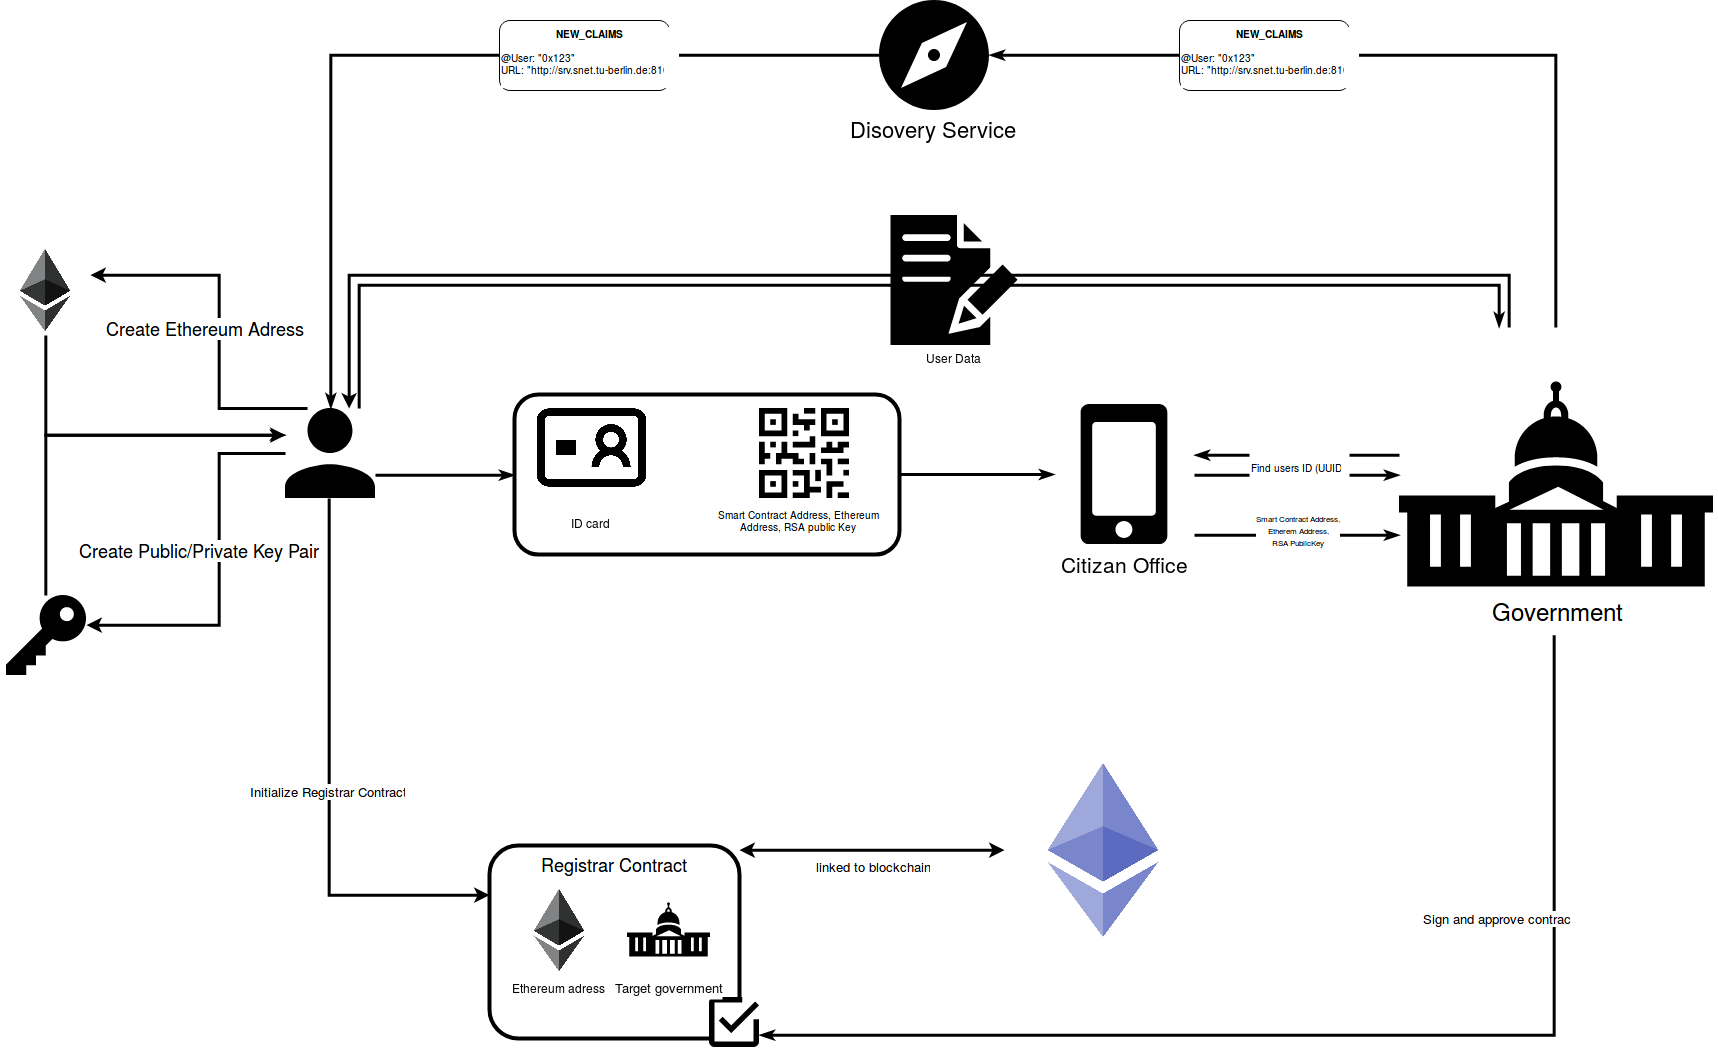
\includegraphics[width=\textwidth]{impl/RegisterContractImpl.png}
\centering
\caption{Implementation of the Register Contract flow. Since it was not possible (time limitations) to include the eID verification mechanism, we implemented the in-person verification. Here the newly registered user has to go the citizen office to show his ID card and to get his ethereum address, RSA public key and smart contract address verified.}
\label{fig:registerContractImpl}
\end{figure}

To start the register process the user services exposes the unsecured resources "Account" which provides action endpoints for login, logout, register and QR-code retrieval (later more on that), where the web client can make a HTTP-POST call to "account/register" with a newly set password.
This call will trigger three main actions:

\begin{enumerate}
\item Creating a 4096-bit security RSA key pair
\item Creating a new wallet containing EC-Key Pair 
\item Setting up the register contract 
\end{enumerate}

\subsubsection{Creating RSA and EC key pairs}
We need the RSA key-pair to later encrypt sensitive data that is send over the blockchain since the blockchain itself is a public ledger and for world readable. The key-pair created by web3j does not provide any confidentiality since the ECDSA (Elliptic Curve Digital Signature Algorithm) can only be used to generate and verify signatures (see section \ref{sec:ecdsa}). So the users creates a 4096-bit strong RSA key pair (step 1.1). So ensure that this key indeed belongs to the newly generated EC key-pair (step 1.2) we generate a signature over the RSA public key with the EC private key and publish this information to the discovery service.

We further also save our keys, password based symmetric encrypted, to the ethereum data directory under \lstinline|{$USER.HOME}/.ethereum/blockchain-identity/|\footnote{The \lstinline{"~/ethereum"} directory is the default directory to save all ethereum related files.}. If the user later logs out, we can simply remove the current RSA and EC keys from memory and if the user logs in again, providing his password, we can decrypt the wallet file using his password and read the RSA and EC keys back in memory. 

The user service application is planned to run locally on the users host machine. This would secure it from outside access. Since we didn’t manage to implement a key recovery mechanism there might be an Denial-of-Service attack vector possible where a malicious application running also locally on the users host machine, call periodically the register-endpoint, preventing the user from accessing his information because his keys gets reshuffled every time. Some could think about disabling this register endpoint after successful creating a key pair, but since this is a prototype under developing this endpoint needs to be open and accessible. The endpoints of the user service are also not secured. We could here also use JWT to secure them and prevent any malicious application from accessing this data. 

\subsubsection{Deploying the register contract}
To now register the user that is bound to his ethereum address we setup a register contract (step 2.). This register contract is a representation of the unverified user and contains no more information then the users ethereum address and a flag if the user is approved by the government. This flag can only be set by the trusted government. 

\subsubsection{Verifying the user}
As shown in figure \ref{fig:registerContractImpl} the user then creates a QR-Code (step 3.) to encode his ethereum address, address of the smart contract and his public key into it.\footnote{It is not necessary to encode the public key into the QR-code at all since the Discovery Service also stores this information, but we can save an additional request from the government side to discover it by providing it in the register flow directly.} The QR-code generation is done with the help of the Xzing library and exposed via an rest endpoint "/account/qr-code". The idea to generate a QR-code is simply that ethereum addresses are quite hard to type and since the user has to go to the citizen office in person he might as well just show is representative QR-code. 

The citizen office verifies that the user is who he claims to be with the use of the provided ID card. The android application build for the purpose of scanning the QR-code, generating a signature over the retrieved information and sending it to the government service, needs further know which user is currently trying to be verified to the system. To do so the citizen office types in the user information found on the ID card, for example given name, family name, etc. to then send a authorized requests to the government which then queries its database for a user with the same information and returns his UUID (step 4.). 

With the retrieved UUID the application can then make a signed POST request to the user resource  and updates the user for his public key, ethereum address and register contract address (step 5.).

\subsubsection{Finalize user registration}
The government uses the information about the user to update the register contract by setting the approval flag (step 6.). Now every party in the system observing the blockchain can verify that the user holding the private key for the ethereum address is indeed verified by the government. If each provider checks that he is only communicating with verified users we are preventing sibyl attacks in the most effective way possible. 

A new signed beat (section \ref{sec:beats}, step 7.1 and 7.2) is created with the event "NEW\_CLAIMS" addressed at the users ethereum address to notify the user to request the government API (section \ref{sec:providerAPI} to retrieve the signed claims stored at the government service about him (step 8.). 

Since a new user is now verified in the system other provider shell also send the user their claims about him. That point was really difficult to implement and was left open for further work since there are open unanswered questions: How do provider assign the new ethereum address of the newly registered user to any costumers of their system (you can not broadcast any user claims over the network because of privacy reasons)? How to ensure that provider send all their claims (since they are not trusted they might be malicious)? 
In the end we said that the user has to manually notify provider about his presents in the system. This could be done by selecting a set of registered providers from the discovery service and broadcasting an “CALL\_FOR\_CLAIMS” event to thous providers. The user would then need to somehow authenticate to the provider by for example login in into their web page and approving his call for claims manually. 

\subsection{Permission Request}
\label{sec:ppr}

\begin{figure}
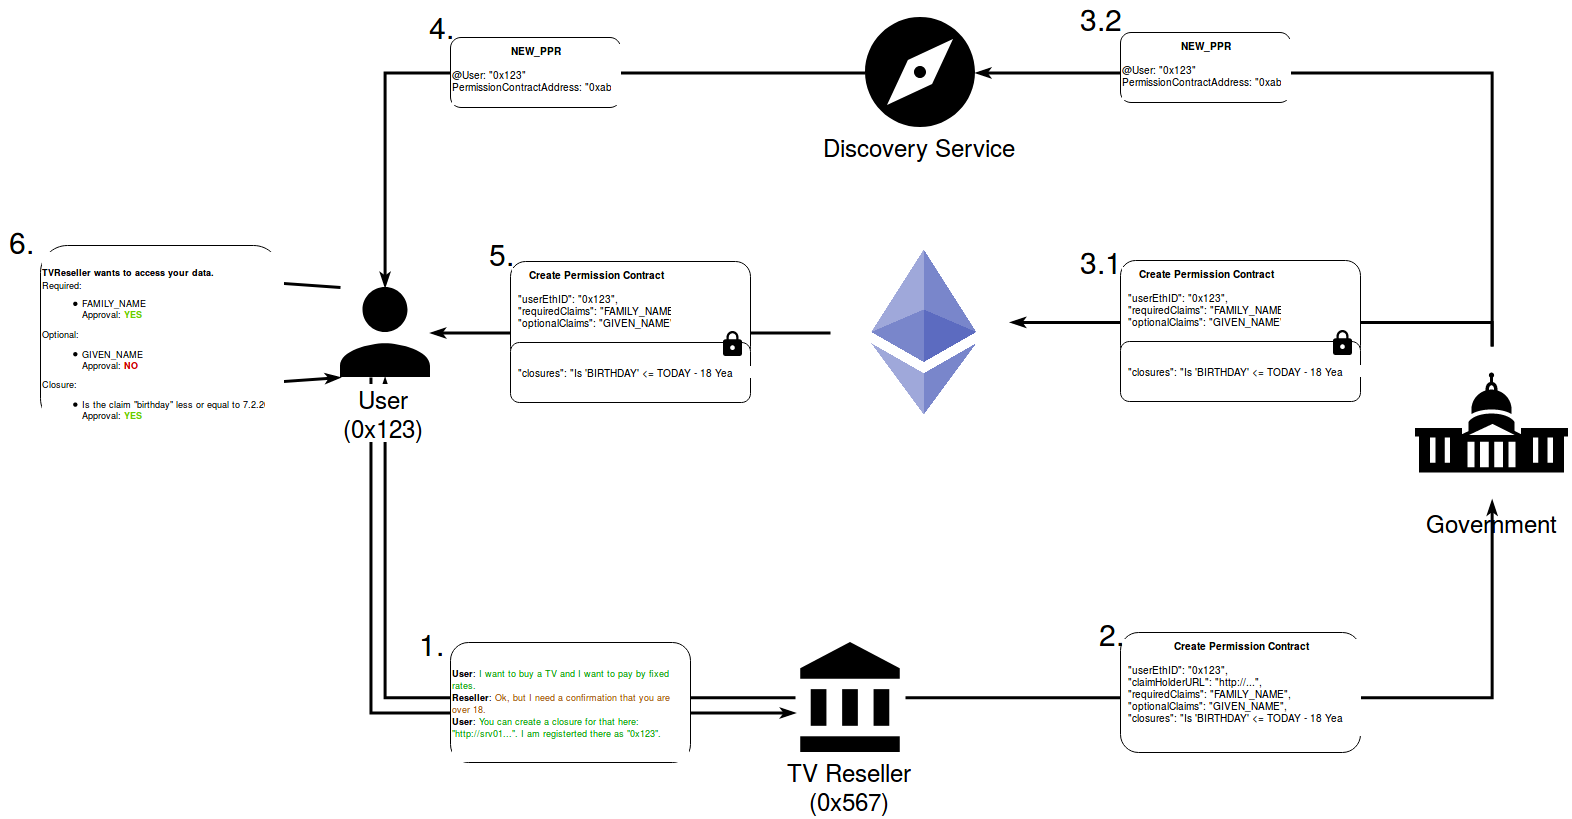
\includegraphics[width=\textwidth]{impl/PPR_closure_1.png}
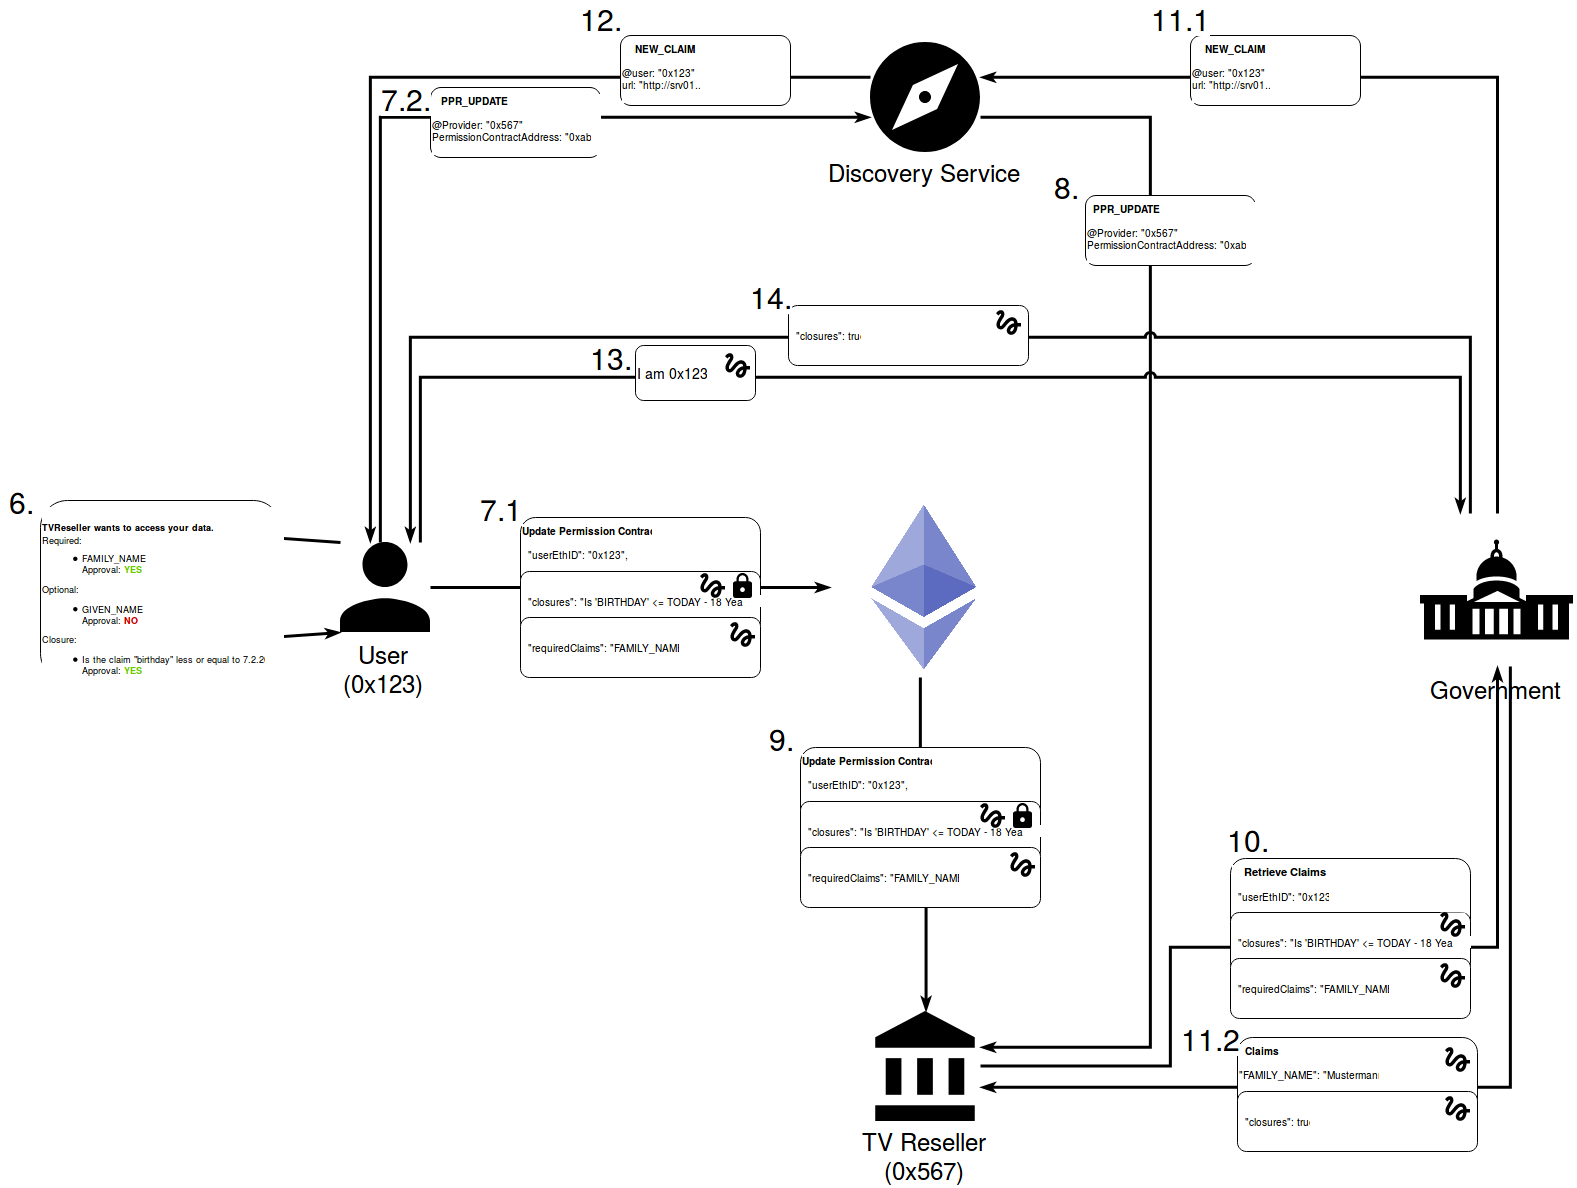
\includegraphics[width=\textwidth]{impl/PPR_closure_2.png}
\centering
\caption{Flow to request permission about GIVEN\_NAME (optional) and FAMILY\_NAME (required) and a closure over the age of the user.}
\label{fig:ppr}
\end{figure}

Located in the core of our project stand the Provider Permission Request (PPR). Its goal is to ensure that every request about the sharing of claims is routed to the user, which can approve or disapprove the information population. With PPR-Contracts it is further possible to see which provider holds which data about which (pseudonymous) user. To implement the PPR flow we need all of the previous introduced technologies since all services need to play together to implement the PPR. 

We start by the provider requesting the user information (step 2.). Please ignore the closure reference in the figure \ref{fig:ppr} it will be explained separately. From the frontend we are receiving the user’s ethereum address, that was populated to the network in the register contract (section \ref{sec:registerContract}), and an URL referencing the provider that is holding the claims that shell be shared (step 1.). The last missing information are the claim IDs that shell be requested. The application differences between required and optional claims. Required claims need to be approved by the user or the whole PPR will be discarded. Optional claims can be partially accepted or rejected by the user, the PPR will still be executed. So the provider sets the claim IDs appropriately and signs this PPR and sends it to the provider holding the claims about the requested user. In return he will retrieve the smart contract address of the created PPR contract. He creates also a PPR meta object that holds the current state of the pending PPR and saves this object in his database. 

The information what claims are known about a user is exposed through an unsecured endpoint. This endpoint is not exposing the values to the claims, rather it only exposes the claim IDs, types and supported operations of this types. We consider this information not critical to protect, since this are the same information anyone can read from the blockchain. Future research can be done in this direction to create a mechanism to protect this information since they might enable to locate valuable targets. 

The government service is a trusted service that can also write to the blockchain. Please note that we can create PPRs to every provider that is able to write to the blockchain. We government service will proceed to process the request, by first verifying the signature and second checking if the requested claims match the claims the targeted user hold.  

In Step 3.1 the government is populating the received information in form of a smart contract to the blockchain. This smart contract is addressed to the user that is the owner of the requested claims. Parallel in step 3.2. the user is notified via a new beat with event “NEW\_PPR”, referencing the recently created smart contract.
This beat gets read by the user in step 4. and processed by retrieving the smart contract from the blockchain in step 5. Since all information about the claims in PPR are unencrypted everyone can ensure that a PPR was created over the defined claims IDs and that the user is now processing the PPR. He is doing so by saving the PPR in his database and creating a new message to notify the frontend that a new PPR was retrieved. In Step 6 the frontend now asks the user for his explicit approval. As mentioned previous a rejection of all required claims would result in a rejection of the PPR itself. It would still be updated in the blockchain so that the requesting provider know that the PPR was rejected. To approve the PPR the user must accept the sharing of all required claims and can decide which optional claims he wants to share as well.  

Upon receiving the information which claims the frontend approved, the user service generates a signature over the claim IDs that were approved. This is done in the form of a signed request over the claim IDs. We need also to include the providers address in to the signature to ensure that the signed request gets not reused by other providers. Finally object mapper is used to translate this object into a JSON string (later needed to send this JSON to the government) and then converting this string into base64 representation (get rid of any non ASCII characters to ensure compatibility with the ethereum serialization) to put it into the blockchain (step 7.1). Unapproved requests will not receive a signature. We are not encrypting this signature in anyway since everybody shell take note that the user approved the PPR entry. This will ensure that the user can not later deny to has approved this PPR entry. To also notify the requesting provider that the user updated the PPR contract, the user service is creating a new beat with event “PPR\_UPDATE” addressed at the provider that initially requested the claims, referencing the updated permission contract (step 7.2). 

The provider registers this beat (step 8.) and can now pull the updated PPR information from the blockchain. He evaluates whether the contract was at all approved (if all required claims were signed) and updates the PPR meta object in his database with the information about approved claims. This object can later be used to display administrator which claims get usually approved and serves further as a permission history for each user. 

Here the implementation and concept slightly differ in two points. First we defined in our concept that the user includes an encrypted hash over the his claims and send them trough the blockchain. Respecting GDPR this in not the way to go. Even if it is a hash and even if it is encrypted, both may be broken in some time, exposing the plain claims in the blockchain were they can not be removed. We then thought about sending the integrity check over the discovery service and retrieve it in step 8. However, building a hash over our claims is not trivial to do and is further evaluated in the evaluation section \ref{sec:untrustedSystem}. We didn’t any integrity check here since the government is currently the only claim holder and also a trusted system. So we trust the system to not tamper with the user data. However, if any other provider then the government would be the claim holder, we would need include this integrity check. 

Second, the user is not generating signed queries that can be used by the provider to select certain claims. There are several reasons running and generating queries was a bad idea. Main argument are object claims. The user service must somehow interpret the request from the provider to build a query out of it. This is not trivial and the queries must support full SQL syntax to cover all use-cases. Another issue is that the government service would likely don’t want to run run user generated queries on its database. First they have to interpret this query and check that it only selects elements (no deletion, no tampering) and second that the query is selecting only attribute from the user that issued the query. 
This would add more logic and would make PPRs much more complex then they have to be. Surely SQL statements can be exploited if user and provider cooperate to attack the government.
However, what we did is building a signature over claim IDs and the provider ethereum address so that the government can use the claim IDs to select them, by building a query by its own. It simplifies the security checks and the query processing overhead. 

To finally retrieve the signed claim values in step 11.2 the provider uses the user signed JSON strings to query the government service for the claim values. The government service on the other hand can verify the signature of the user and so knows that the user explicitly approved to share the given claims. He also verifies that the requesting provider is indeed the provider the user granted permission (remember that the provider address is also signed by the user). If all requirements are fulfilled the signed claims matching the claim IDs in the requests are returned (step 11.2).

Here ends the permission request. The following steps are only an extension to handle closure requests accordingly. They will be described in the next section.     

\subsection{Closures}
\label{sec:closure}
Closures are boolean expressions that do not reveal information about the actual claim value. For example a common closure is “Is Bob over 18?”. We can answer this question with yes or no but we do not reveal Bobs birthday. However we see the question as a semi-critical personal information which needs to be protected. Semi-critical since it is not a essential personal information and it is not fatal if the encryption gets broken in the future and we can not remove the closure from the blockchain. However, we encrypt the compared value, so that some only see the closure “Is Bob over $\bullet\bullet\bullet$?”. In this case it might be easy to guess, but the point is that closures in general remain public visible, while the compared value remains secret. So everybody can still see that an exchange happened, but does can not gain any new information about Bob. 

The closure flow is tightly bound to the permission request flow. They both are displayed in the figure \ref{fig:ppr}.  We start off by step 1. where the TV reseller wants a closure over the users age and wants to know if the user is over 18 years old. As already known from the PPR flow the provider does now request the government service for the respective closure. 

\noindent A closure in code form consist of three values: 
\begin{itemize}
\item \textbf{claim ID}: References the claim that shell be used for the closure evaluation. 
\item \textbf{claim operation}: Defines a logical operation that shell be used as comparator. 
\item \textbf{static value}: The value which shell be used for comparison. 
\end{itemize}

The type of the requested claim defines which operations are supported (appendix \ref{appendix:claimOperation}) and sets the type that the static value needs to have. Indeed it makes no sense to compare a string to a number. Claims from type objects are not yet supported for closures since it is not easy to find a unique set of operations that are executable on them. We thought about using a JSON query language that let us query arbitrary JSON objects and compare their properties to other values. First this seemed like a good and powerful solution, but later it was clear that is not piratical since the user needs to understand the expressions to either approve or reject them. We have no chance to parse the JSON query language to a user friendly representation. Also this query language would introduce new attack vectors at user claims and may also trick the user to approve a query that may select something complete different then that, what the user though he would approve. Defining a static set of operations in such a inflexible fashion as we did, allowed us to parse a user friendly question out of it, so that every user understands what is requested. Further we also have the power to limit the expression language in that kind that no new attack vectors are introduced and expressions will not have any side effects. Simplicity is less powerful but easier to maintain and so increases security. 

The government, as holder of the claim value, can verify that the claim operation and static value matches the type of the requested claim target. If all checks succeeded it will encrypt the static value using a newly generated symmetric session key (AES, 256 bit). To do so the static value will be converted into a byte representation and then encrypted. To now send the session key securely over to the user it is encrypted asymmetrically with the public key of the user (RSA, 4096 bit). We archive forward secrecy here since the session key is a one time session key that is discarded after usage. Our closure is now secured and ready to be put into the blockchain in step 3.1. 

In step 5 the user extracts the closure from the blockchain by first decrypting the session key with his RSA private key. He now can decrypt the static values of the closure requests. After that is done we can request the claim values from the database of the user to evaluate the closure expression. This is done by simply evaluating the claim value with the given claim operation and the given static value. We further can now compute the user friendly description of the closure expression. Since we assigned each claim operation a lingual expression (see appendix \ref{appendix:claimOperation}), we have all components together to build up a question. To know if a person is over 18 years old an description as in figure \ref{fig:closureDescribtion} is generated.

\begin{figure}
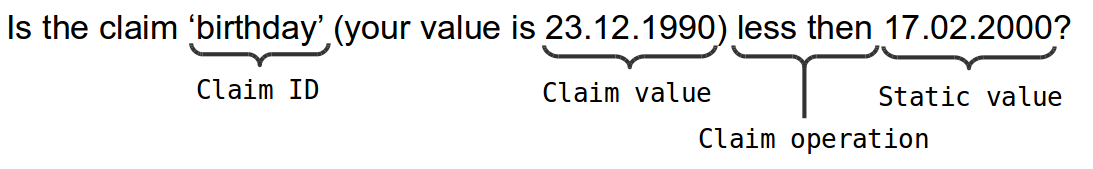
\includegraphics[width=0.6\textwidth]{impl/closure_describtion.png}
\centering
\caption{Components of a closure description that is generated to create a user friendly literal expression.}
\label{fig:closureDescription}
\end{figure}

The user can now decide to either approve or reject this closure. For each approved closure the closure is signed and the static value is again encrypted with a newly generated session key which is then again asymmetrically encrypted. The difference now is that the contract is addressed to the requesting provider, so the static values need to be encrypted with the public key of the requesting provider. Since the user may not know this public key he can discover it. This is simply done by querying the discovery service that is holding all public keys to ethereum address mappings. To validate that the retrieved public key indeed belongs to the ethereum address of the requesting provider, the user service verifies the signature of the received entry and compares the computed ethereum address with the requested provider’s ethereum address. The PPR is updated with the new information (step 7.1) and a new beat is created to notify the provider (step 7.2). 

At this point the closure flow quite similar to that of the PPR. From the updated permission contract  the closure is decrypted using the private key of the provider (step 9.) and the signatures of the closures are verified to respond accordingly to the user on an error case. If the provider would forward this signature without validating the government service would verify the signature, run into an error and the trust in the requesting provider would be reduced since he tried to fake an signature. 

As already known from the PPR the signatures over the closure request is used to request a real closure (step 10.). Beside the claim ID, claim operation and static value, a closure in its final form, contains additional the following values: 

\begin{itemize}
\item \textbf{Creation date:} The date the closure was created. Parties may use this value to decide whether they are willing to accept the closure. A fixed threshold is not defined since different closures can be valid for different time episodes. 
\item \textbf{User’s ethereum address:} The address of the user this closure is about. Closures are not addressed at a specific provider and so representing a universal verified statement. 
\item \textbf{Expression result:} The result of the closure evaluation. The evaluation result is bound to the claim value of the user at the time of creation of this closure. So it will not change if the user for example become full age. 
\item \textbf{Issued provider ethereum address:} The provider that created the closure. This does not need to be the government, since every entity may produce closures. However, the trust in the closure depends on the trust established in the issuing provider. 
\item \textbf{Signature:} The signature of the issuing provider. It is generated over all the above values to ensure their integrity and authenticity. 
\end{itemize} 

To finally provide the user with the power of self distributing the newly generated closures are also forward to the user. Closures are saved as an additional field in the claim object of a user, which enables us to simply create a new beat with the message of "NEW\_CLAIMS" (step 11.1). This will trigger the user service to use the (in the beat) provided URL and its signature to query the government service for new claims (step 13.) and retrieve the update claims with the receptive closures (step 14.). If an other provider requests the same closure the user can simply provide the closure to him. The provider verifies the signature and decides whether the closure is fresh enough or an update is needed. In the last case the whole process will start again. 

\subsection{Summary}
\label{sec:coreSummary}
Due to time limitation it was not possible to implement the change claim concept. But since all core-components, required to implement the change claim work flow, are already present in the system, we are not so far away from getting this implemented.

To sum up the implementation in the backend, we created a powerful and scalable solution of provider – user interactions. A unified provider API lets provider talk to each other in a well defined manner. This API is easily expendable to add further functionality to the system. Further the backend operates though well defined interface to the other components like the REST API to the frontend and the EBA interface to the ethereum blockchain. Besides the component definition we explained and discussed how signatures are generated and validated and which challenges arise in a distributed system by generating signatures over arbitrary objects.  We shortly examined the drawbacks of object to string conversions and how to overcome this obstacles. Further the design of closures and claims were explained, how closure expressions are evaluated and how to produce a user friendly lingual expression out of a logical condition. Finally we explained the flow of registration, permission granting and closure requesting in detail and pointed out the code parts where the previous introduces methods where used. When the implementation differed from the concept, we argued why the implementation was different and why a simpler implementation increases security. 

% ------------------------ EBA -----------------------------

\section{Ethereum Blockchain Adapter - EBA}
\label{sec:eba}

% ------------------------ FRONTEND -----------------------------

\section{Frontend}
\label{sec:frontend}


\subsection{Motivation}

The frontend is the interface for both users and third parties to interact with the system.
The user interfaces' focus is to purely show information and an appropriate way and have a bare and minimal design
in order to not get distracted by other features.
Further, responsiveness is a key aspect to make sure that the system can be used on any device. This for one makes the
system more attractive to use but also grants the user a higher accessibility to his sovereignty.

\subsubsection{Tools and Technologies}

As previously described, the backend read and write access is implemented with a RESTful API.
With ReactJS as a frontend library we improved the development speed of the user interfaces so we could purely focus
on functionality.
For the actual communication and updating of state we used Redux-Saga, which is a state management storage with a heavy focus
on data fetching and asynchronous tasks, which comes in handy for this application.

Besides ReactJS and Redux-Saga we further committed us to the following technology stack:

\begin{itemize}
\item material-ui\footnote{\url{https://material-ui-next.com/}}: A ReactJS implementation of Google's Material Design.
\end{itemize}

Further the following technologies are used for testing:

\begin{itemize}
\item Jest\footnote{\url{https://facebook.github.io/jest/}}: A common Javascript testing framework
\item Enzyme\footnote{\url{http://airbnb.io/enzyme/}}: A ReactJS testing framework.
\end{itemize}

\subsection{Third party}

As a third party the interface is focused on requesting data of a user. There are input fields for the user's Ethereum address
and the parameters that can be requested. Those are claims and closures, which are described more in-depth in the concept.
The third party can explicitly select claims and set them to either required or optional.
Further closures can be constructed to be humanly readable by selecting predefined terms which result in a boolean result,
such as "Is your birth date 02.02.2002 after 05.05.2005?". Its purpose is that the user can easily understand the query.
Whenever the user interface triggers events to the backend, small snack bars inform the third party about the data exchange.

\subsection{User}
\label{sec:user}

The user interface is the main part of the application and consists of 4 minimally design sections, general information,
claims, requests, and permission history. The user has the ability to show the sections or fold them together if needed.
Whenever events that target the backend are fired, the user is informed by a notification with a snack bar on the top of
the display.

\subsubsection{General information}

The first section is about general information of the user, e.g. the own Ethereum Address and the option to verify yourself
at the government by scanning a QR-code with the mobile app. The user has the ability to hide and show the qr code.

\subsubsection{Claims}

The second section hold a table with all the currently existing and verified claims by the system. There the user has an
overview and can check his data and by whom is was approved.

\subsubsection{Requests}

In the third section we show incoming requests. Those requests stem from a third party which was approved by the government
and contain asking for permissions for required claims, optional claims and closures. The user can then approve or deny
each item that was asked for and send his answer. If a request is answered, it disappears from the section.

\subsubsection{Permission History}

The last section show all responses to already answered permission requests in the past. It is shown as a table since the
user cannot directly change its data and only get informative data from previous data exchanges and permission grants.

\subsection{Mobile App}

The mobile app has the sole purpose of using the phone's camera to scan the user's QR-code and hereby approve the user in
the system.

\subsection{Summary}
\label{sec:frontendSummary}

All in all the frontend is feature complete and would need to be extended with more features such as changing claims in
the future. Due to the nature of the framework being used, ReactJS, it is highly flexible and can be easily extended by
adding new components and make a newly interwoven prototype with it.

% ------------------------ DATABASE -----------------------------

%Database part
%-motivieren wieso couchbase
-%spring anbindung
%-schemaless storage gut für unsere claims
-%könmnen signierte jsons direkt in die datenbank speichern, und genauso auslesen -> kein transfer in andere repräsentation
%-couchbase mobile coming soon(tm)
%-begrenzter speicher -> daher nur eine couchbase instanzt, anstatt eine instanz pro "beteiligter person"
%-kaum indizes, da zu weniug speicher
%--queryen ist zu langsam
%--couchbase frass zu viel speicher und hat andere docker container vernichtet
%

\section{Database}
\label{sec:database}

We selected Couchbase as our database management system. In the following sections we will motivate this decision.

\subsection{Motivation}
\label{sec:databaseMotivation}
During the design stage of \projectName{} we focussed on designing the flow of transactions and information before deciding on a definitive database solution.
After finalizing our ideas for how transactions and claims are structured we started evaluating multiple database alternatives.
We started by establishing a small set of features we deemed necessary and indispensable. These features were:
\begin{itemize}
\item \label{db_req_one}
Storage that is deployable on mobile devices such as smart phones and tablets, since users hold their own claims.
\item \label{db_req_two}
Free licensing structure for development.
\item \label{db_item_three}
Lightweight storage for user side claim management (section \ref{db_req_one}).
\item \label{db_req_four}
Schemaless files since claim structure can vary by claim type and value. Removing the need for strict typography of data attributes as used in RDBMS (Relational Database Management Systems)
\item \label{db_req_five}
Possibility of directly writing our objects into a database without the need for transforming them, including cryptographically signed objects.
\item \label{db_req_six}
In order to keep the workload manageable we decided on using a DBMS that we were already familiar with.
\item \label{db_req_seven}
Since we are using Springboot as our backend framework it is imperative that the chosen DBMS is compatible.
\end{itemize}

\subsection{Alternatives}
\label{sec:databaseAlternatives}
Afterwards we checked the various types of data storage possibilities and we rated them according to our criteria.

\subsubsection{Relational Database Management Systems (RDBMS)}
\label{databaseRDBS}
\begin{itemize}
\item \label{rdbms_req_one} \textbf{Mobile deployability:}
One of the most popular mobile databases is SQLite which follows the typical RDBMS schema.\cite{dbcharts} Therefore we strongly considered SQLite as our leading RDBMS alternative.
\item \label{rdbms_req_two} \textbf{Licensing:}
SQLite is public domain and therefore the licensing is as unobstructive as can be.
\item \label{rdbms_item_three} \textbf{Lightweightness:}
SQLite is already used to power an enormous amount of mobile and embedded applications\cite{sqlite}
\item \label{rdbms_req_four} \textbf{Schemaless:}
Just as any other RDBMS SQLite however is not schemaless.
\item \label{rdbms_req_five} \textbf{Transformation:}
Since SQLite is not schemaless we would have had to develop a transformation scheme to map our incoming data to specific columns.
\item \label{rdbms_req_six} \textbf{Familiarity}
Working with SQLite is closely related to working with other RDBMS and therefore we would be familiar with that working environment.
\item \label{rdbms_req_seven} \textbf{Compatibility}
SQLite is not compatible with springboot out of the box.
\end{itemize}
In conclusion SQLite as our preferred RDBMS was simply not an option for implementation purposes.

\subsubsection{Key-value store}
\label{databaseKeyValueStore}
\begin{itemize}
\item \label{kv_req_one} \textbf{Mobile deployability:}
We found LevelDB as an alternative to a mobile deployable key value store.
\item \label{kv_req_two} \textbf{Licensing:}
LevelDB comes with a fairly lax licensing scheme only requiring the licensee to not alter the license file in any way, shape or form. Additionally the license file is to be displayed as written by the licenser.
\item \label{kv_item_three} \textbf{Lightweightness:}
LevelDB is a specialized key value store developed by google for their android operating system.This ensures that LevelDB is mobile ready out of the box.
\item \label{kv_req_four} \textbf{Schemaless:}
Since LevelDB is a simple key value store it can be considered to be schemaless. It simply saves a combination of two byte arrays with arbitrary length as key:value.
\item \label{kv_req_five} \textbf{Transformation:}
Due to LevelDB's nature we would have had to transform our objects into a fitting encoding for saving and retrieving purposes.
Furthermore LevelDB has no indexing at all and therefore we would have had to design an intelligent retrieval scheme for specific entries.
\item \label{kv_req_six} \textbf{Familiarity:}
None of us has even worked with LevelDB before.
\item \label{kv_req_seven} \textbf{Compatibility:}
Springboot is compatible with apache camel which is a LevelDB based extension.
\end{itemize}
No indexing and impossiblity of querying elimited LevelDB from the list of alternatives.

\subsubsection{Document based DBMS}
\label{databaseDBMS}
\begin{itemize}
\item \label{doc_req_one} \textbf{Mobile deployability:}
Couchbase lite is a couchbase based mobile derivative with upcoming mobile convergence. Meaning that depending on the use case they are interchangeable without having to modify the codebase.
However at the start of the project couchbase lite was still in pre-release forcing us to fall back to non-mobile couchbase service. However because of the upcoming mobile convergence it wouldn't hinder development at all.
Exchanging couchbase with couchbase lite would just be a simple switch in the configuration files.
\item \label{doc_req_two} \textbf{Licensing:}
Couchbase lite is licensed with Apache2.0 and therefore is not infringing on our projects aims.
\item \label{doc_item_three} \textbf{Lightweightness:}
Couchbase lite is deployable on all modern operating systems including but not limited to iOS, Android and Windows.
\item \label{doc_req_four} \textbf{Schemaless:}
Couchbase is a schemaless storage solution focussing on writing so called documents containing keys and values. These documents follow the JSON schema and therefore are a perfect fit for a web focussed project dealing with a state of the art frontend and backend.
\item \label{doc_req_five} \textbf{Transformation:}
Since it is a document driven database it is possible to directly store our signed JSONs into the database.
\item \label{doc_req_six} \textbf{Familiarity}
Because of various other projects and work commitments we are very familiar with document based communication and document based storage solutions in particular.
\end{itemize}
Because of the aforementioned reasons we chose couchbase as our primary data storage solution. Changing it to couchbase lite as soon as it is released in a finalized stable long term supported version.

\subsection{Deployment}
One of couchbases particularities is the bucket design. A bucket is meant quite literally, as you can put whatever data you want into it and save it until changed or deleted. Couchbase itself also offers very comfortable retrieval and updating mechanisms by
offering a built-in upsert method. Which either retrieves an entity and overwrites it with a new verison or creates a new document from the given content.
Our first approach was to create a bucket for each entity that is part of the system to simulate the envisioned system as closely as possible. However extreme memory limitations soon made us realize that we had to abandon that concept for the time being and adapt a more pragmatic approach.
We created a single bucket for all our database persistence needs. Since couchbase allows the saving of different documents to the same bucket this was not a problem.
To add on to our memory woes we weren't able to create all of the required indices making querying slow at times and impossible at maximum memory utilisation.
Lastly since we packaged each component into a seperate docker container, with the couchbase container utilising the majority of the memory, we had memory conflicts on our hands leading to unexpected container shutdowns.

\subsection{Summary}
\label{sec:databaseSummary}
Couchbase enabled us to save our claims as we envisioned them without having to develop transformation and mapping methods.
Additionally it allowed us to directly save signed documents further simplifying our database management.
